%
%  kant.one
%
%  Created by Mark Eli Kalderon on 2007-08-04.
%  Copyright (c) 2007 Mark Eli Kalderon. All rights reserved.
%
%  Beamer

% Definitions and macros
\newcommand{\change}{\textcolor{blue}{\textbf{CHANGE SLIDE}}}
\newcommand\myauthor{Mark Eli Kalderon} 
\newcommand\mytitle{Introduction to Moral Philosophy}
\newcommand\mysubtitle{Kant}
\newcommand\myinstitution{University College London}
\newcommand\myurl{http://markelikalderon.com/teaching}

% Packages specific to lecture notes
\mode<article>{
	\usepackage{palatino}
}

% Packages specific to beamer presentation
\mode<presentation>{
	\usetheme{Darmstadt}
	\setbeamercovered{transparent}
	\pgfdeclareimage[height=0.5cm]{university-logo}{../../graphics/logo_sml_blk}
	\logo{\pgfuseimage{university-logo}}
}

% Packages common to lecture notes and beamer presentation
\usepackage{pgf}
\usepackage{tikz}
\usepackage{hyperref}

\setjobnamebeamerversion{kant.one.beamer}

\title{\mytitle}
\subtitle{\mysubtitle}

\author{\myauthor\\
\url{\myurl}}
\institute{\myinstitution}

% \date[Short Occasion] % (optional)
% {Date / Occasion}

\begin{document}

\frame{\maketitle}

\section{The Project of the Groundwork}\label{sec:the_project_of_the_emph_groundwork_} % (fold)

Kant’s project in the \emph{Groundwork} is ``the search for and establishment of the \emph{supreme principle of morality}'', that is, the moral law (G 4:392). There are two questions:

\begin{enumerate}
	\item What is the supreme principle of morality?
	\item Does the supreme principle of morality exist?
\end{enumerate}

The first question, ``What is the supreme principle of morality?'', is answered in the first two sections of the \emph{Groundwork}. The second question, ``Does the supreme principle of morality exist?'', is only answered in the third section.

% \textbf{See Figure~\ref{fig:slide1}.}
% 
% \begin{figure}[ht]
%     \begin{center}
%         \includeslide[height=5cm]{slide1<1>}
%     \end{center}
%     \caption{The Project}
%     \label{fig:slide1}
% \end{figure}

\frame<presentation>[label=slide1]{
    \frametitle{The Project}
        \begin{columns}
            \begin{column}{3cm}
                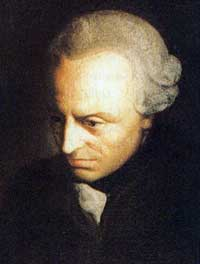
\includegraphics[height=4cm]{../../graphics/kant.jpg}
            \end{column}
            \begin{column}{7cm}
                The ``search for and establishment of the supreme principle of morality''.\\
                Two questions:
                \begin{enumerate}
                    \item What is the supreme principle of morality?
                    \item Does the supreme principle of morality exist?
                \end{enumerate}
            \end{column}
        \end{columns}
}

The first section provides a provisional answer: The supreme principle of morality is the categorical imperative represented by the Formula of Universal Law. The second section provides a more complete answer: The categorical imperative is represented by a system of three formulas (two of which have variant formulations):\\

\textbf{FIRST FORMULA}
\begin{itemize}
	\item \emph{The Formula of Universal Law}: ``Act only in accordance with that maxim through which you can at the same time will that it become a universal law.'' (G 4:421; 4:402)
	\item \emph{The Formula of the Law of Nature}: ``Act as if the maxim of your action were to become by your will a universal law of nature.'' (G 4:421; 4:436)
\end{itemize}
\textbf{SECOND FORMULA}
\begin{itemize}
	\item \emph{The Formula of Humanity}: ``So act that you use humanity, whether in your own person or that of another, always at the same time as an end, never merely as a means.'' (G 4:429; 4:436)
\end{itemize}
\textbf{THIRD FORMULA}
\begin{itemize}
	\item \emph{The Formula of Autonomy}: ``\ldots the idea of the will of every rational being as a will giving universal law.'' (G 4:431; 4:432)
	\item \emph{The Formula of the Kingdom of Ends}: ``Act in accordance with the maxims of a member giving universal laws for a merely possible kingdom of ends.'' (G 4:439; 4:433; 4:437; 4:438)
\end{itemize}

Kant claims that the three formulas represent the same principle and that they differ only in representing different aspects of that same principle (G 4:436–437). Kant also claims that for \emph{appraisal} of an action the first formula is best, but that for \emph{access} to the moral law the three formulas should be applied to one and the same action thereby bringing the moral law closer to intuition and thereby feeling.

% \textbf{See Figure~\ref{fig:slide2}.}
% 
% \begin{figure}[ht]
%     \begin{center}
%         \includeslide[height=5cm]{slide2<1>}
%     \end{center}
%     \caption{The System of Three Formulas}
%     \label{fig:slide2}
% \end{figure}

\frame<presentation>[label=slide2]{
    \frametitle{The System of Three Formulas}
        \begin{columns}
            \begin{column}{3cm}
                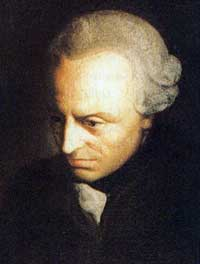
\includegraphics[height=4cm]{../../graphics/kant.jpg}
            \end{column}
            \begin{column}{7cm}
                \small{\textbf{FIRST FORMULA}}
                \begin{itemize}
                	\item \small{\alert{The Formula of Universal Law}}
                	\item \small{\alert{The Formula of the Law of Nature}}
                \end{itemize}
                \small{\textbf{SECOND FORMULA}}
                \begin{itemize}
                	\item \small{\alert{The Formula of Humanity}}
                \end{itemize}
                \small{\textbf{THIRD FORMULA}}
                \begin{itemize}
                	\item \small{\alert{The Formula of Autonomy}}
                	\item \small{\alert{The Formula of the Kingdom of Ends}}
                \end{itemize}
            \end{column}
        \end{columns}
}

The conclusions of the first two sections are conditional: If the supreme principle of morality exists, it must have a certain character. The existence of the supreme principle of morality is only established in the third section. There Kant argues that the supreme principle of morality as represented by the Formula of Autonomy is only valid for the human will just in case it is free and that in order to act at all the freedom of the will must be presupposed (G 4:447–448). Thus while Kant does not \emph{demonstrate} the existence of the supreme principle of morality, he nevertheless argues that we must presuppose its existence if we are to act at all.

% \textbf{See Figure~\ref{fig:slide3}.}
% 
% \begin{figure}[ht]
%     \begin{center}
%         \includeslide[height=5cm]{slide3<1>}
%     \end{center}
%     \caption{Does the Supreme Principle of Morality Exist}
%     \label{fig:slide3}
% \end{figure}

\frame<presentation>[label=slide3]{
    \frametitle{Does the Supreme Principle of Morality Exist}
        \begin{columns}
            \begin{column}{3cm}
                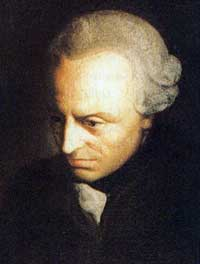
\includegraphics[height=4cm]{../../graphics/kant.jpg}
            \end{column}
            \begin{column}{7cm}
                While Kant does not \alert{demonstrate} the existence of the supreme principle of morality, he argues that we must presuppose its existence
            \end{column}
        \end{columns}
}

% TODO: Add some remarks about the structure of the Groundwork

\textbf{See Figure~\ref{fig:slide4}.}

\begin{figure}[ht]
    \begin{center}
        \includeslide[height=5cm]{slide4<1>}
    \end{center}
    \caption{The Plan of the Groundwork}
    \label{fig:slide4}
\end{figure}

\frame<presentation>[label=slide4]{
    \frametitle{The Plan of the Groundwork}
        \begin{columns}
            \begin{column}{3cm}
                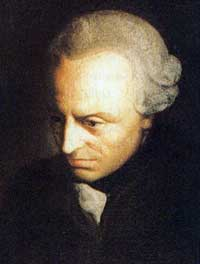
\includegraphics[height=4cm]{../../graphics/kant.jpg}
            \end{column}
            \begin{column}{7cm}
                \begin{itemize}
                    \item \alert{First Section}: Transition from common moral rational to philosophic moral cognition
                    \item \alert{Second Section}: Transition from popular moral philosophy to metaphysics of morals
                    \item \alert{Third Section}: Final step from metaphysics of morals to critique of pure reason
                \end{itemize}
            \end{column}
        \end{columns}
}



% section the_project_of_the_emph_groundwork_ (end)

\section{The Value of the Good Will}\label{sec:the_value_of_the_good_will} % (fold)

\emph{Groundwork} I begins with the startling pronouncement:

\begin{quote}
	It is impossible to think of anything at all in the world, or indeed even beyond it, that could be considered good without limitation except a good will (G 4:393).
\end{quote}

Kant seeks to elicit our assent to this pronouncement by comparing the good will with other kinds of goods:

\begin{itemize}
	\item Gifts of Nature
        \begin{itemize}
        	\item \emph{Talents of Mind} such as understanding, wit, and judgment
            \item \emph{Qualities of Temperament} such as courage, resolution, and perseverance
        \end{itemize}
    \item Gifts of Fortune
    \begin{itemize}
	    \item power, riches, honor, health
        \item happiness understood as ``complete well being and satisfaction with one’s condition'' (G 4:393)
    \end{itemize}
\end{itemize}

Gifts of nature are not unconditionally good but are good only under certain conditions. Thus, gifts of nature can be evil and harmful if the will that makes use of them is not good. Even secondary virtues such as moderation, self-control, and calm reflection, can be extremely evil if used by a bad will (as when the coolness of a scoundrel not only makes him more dangerous but also more abominable).

Gifts of fortune are not unconditionally good but are good only under certain conditions. Thus, gifts of fortune can be evil and harmful if the will that makes use of them is not good.

Even the value of happiness is conditional on the person’s possession of a good will. Kant provides two arguments.

\begin{enumerate}
	\item First, happiness can corrupt: Happiness has a tendency to produce boldness and even arrogance. Kant’s thought seems to be this: Given human nature, persons have a tendency, when happy, to believe that they deserve to be happy whether or not they in fact deserve to be. Moreover, in the appropriate circumstances, such an arrogant delusion can lead to imprudent action or even moral evil. However, a good will can correct the corrupting influence of happiness by acting only on those principles consistent with universal ends determined by pure practical reason.
	\item Second, the prosperity and happiness of a person without a good will can give no pleasure to an impartial rational spectator. (Notice the sentimentalist form of argument. Like Hume, Kant was influenced by Hutcheson’s sentimentalism and was himself a sentimentalist during the pre-critical period.)
\end{enumerate}

From these two arguments, Kant further concludes:

\begin{quote}
	\ldots a good will seems to constitute the indispensable condition even of worthiness to be happy. (G 4:393)
\end{quote}

% \textbf{See Figure~\ref{fig:slide5}.}
% 
% \begin{figure}[ht]
%     \begin{center}
%         \includeslide[height=5cm]{slide5<1>}
%     \end{center}
%     \caption{Goods Other Than the Good Will}
%     \label{fig:slide5}
% \end{figure}

\frame<presentation>[label=slide5]{
    \frametitle{Goods Other Than the Good Will}
        \begin{columns}
            \begin{column}{3cm}
                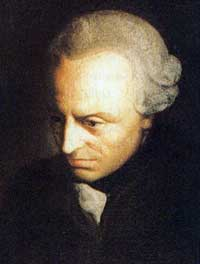
\includegraphics[height=4cm]{../../graphics/kant.jpg}
            \end{column}
            \begin{column}{7cm}
                \textbf{GIFTS OF NATURE}
                \begin{itemize}
                    \item \alert{Talents of Mind}: understanding, wit, judgment
                    \item \alert{Qualties of Temperament}: courage, resolution, perserverance
                \end{itemize}
                \textbf{GIFTS OF FORTUNE}
                \begin{itemize}
                    \item power, riches, honor, health
                    \item happiness understood as ``complete well being and satisfaction with one's condition'' (G 4:393)
                \end{itemize}
            \end{column}
        \end{columns}
}


Gifts of nature or fortune are not unconditionally good but are good only under certain conditions. What are the conditions under which a gift of nature or fortune is good? According to Kant, the value of gifts of nature or fortune are conditional on their use by a good will.

Unlike gifts of nature or fortune, the good will is unconditionally good. The value of a good will does not even depend on what it accomplishes or on its fittingness to attain some independently given end:

\begin{quote}
	Even if by a special disfavor of fortune or by the niggardly provision of a stepmotherly nature, this will should wholly lack the capacity to carry out its purpose—if with its greatest efforts it should achieve nothing and only the good will were left (not, of course, as a mere wish but as the summoning of all means insofar as they are in our control)---then, like a jewel, it would still shine by itself, as something that has full worth in itself. Usefulness or fruitfulness can neither add anything to its worth nor take anything away from it. Its usefulness would be, as it were, only the setting to enable us to handle it more conveniently in ordinary commerce or to attract to it the attention of those who are not yet expert enough, but not to reommend it to experts or to determine its worth (G 4:394)
\end{quote}


Even if a good will lacked the capacity to carry out its purpose (because it lacked the requisite gifts of nature or fortune) it would still have an unconditional value.

Moreover, the value of a good will is incomparably higher than the value of happiness and, presumably, any other gift of nature or fortune no matter how valuable they are. The good will is more valuable than any individual gift of nature or fortune no matter how valuable they are on their own terms. Indeed the good will is more valuable than any aggregate of gifts of nature or fortune: No combination of health, wealth, happiness, etc., is in aggregate more valuable than a good will. The value of a good will will outrank the value of gifts of nature or fortune no matter how valuable they are on in isolation or aggregate.

The good will thus has three distinguishing features:

\begin{enumerate}
	\item The good will is the indispensable condition for the value of other kinds of goods.
	\item The good will is the only kind of thing that is unconditionally good.
	\item The value of a good will is incomparably higher than the value of any other kind of thing whether in isolation or aggregate.
\end{enumerate}

Moreover, while Kant has not defined the good will, he has offered a partial characterization of the good will in terms of the role it plays:

\begin{quote}
	The good will acts consistently from the principles of pure practical reason and so corrects the influence of gifts of nature or fortune by adjusting their use to the universal ends determined by pure practical reason.
\end{quote}

This characterization is formal since we don’t know what these principles are, and so don’t know how persons with a good will actually behave.

% \textbf{See Figure~\ref{fig:slide6}.}
% 
% \begin{figure}[ht]
%     \begin{center}
%         \includeslide[height=5cm]{slide6<1>}
%     \end{center}
%     \caption{The Value of the Good Will}
%     \label{fig:slide6}
% \end{figure}

\frame<presentation>[label=slide6]{
    \frametitle{The Value of the Good Will}
        \begin{columns}
            \begin{column}{4cm}
                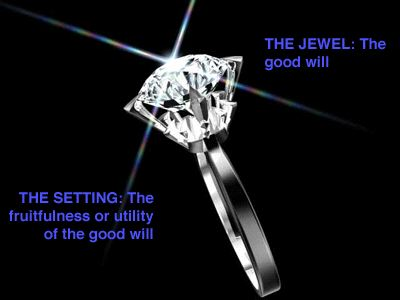
\includegraphics[width=5cm]{../../graphics/diamond.jpg}
            \end{column}
            \begin{column}{6cm}
                \begin{enumerate}
                    \item The good will is the precondition for all good
                    \item Only the good will is unconditionally good
                    \item The value of the good will is incomparably higher than the value of any gift of nature or fortune no matter how valuable they are in isolation or aggregate
                \end{enumerate}
            \end{column}
        \end{columns}
}

In the \emph{Preface}, Kant describes the argument of the first section as a transition from common rational to philosophic moral cognition. We can begin to understand Kant’s strategy given his discussion of the value of a good will.

Common rational moral cognition is the unreflective, practical knowledge of the rational standards that everyone must use in moral reasoning and judgment. Common rational moral cognition is \emph{unreflective} since such knowledge is not based on reflection. Common rational moral cognition is \emph{practical} since it consists in knowing how to act in accordance with such principles.

\begin{quote}
	\ldots there is accordingly, no need for science and philosophy to know what one has to do in order to be honest and good, and even wise and virtuous. (G 4:404)
\end{quote}

Common rational moral cognition is pre-philosophical knowledge of rational standards that every rational being must use in moral reasoning and judgment. Since it is pre-philosophical, common rational moral cognition is subject to philosophical clarification and correction.

Kant’s strategy in the first section, then, is to convert this unreflective, practical knowledge into reflective, theoretical knowledge.

The startling pronouncement that inaugurates the first section raises a question about this strategy:

\begin{quote}
	It is impossible to think of anything at all in the world, or indeed even beyond it, that could be considered good without limitation except a good will. (G 4:393).
\end{quote}

This is not a common sense moral claim and not one that every person possessing common rational moral cognition would immediately assent to. Indeed this seems to be a philosophical claim that, if true, would represent reflective, theoretical knowledge. So has Kant abandoned his avowed strategy right at the very beginning?

To see that Kant hasn’t, it is important to recognize common rational moral cognition is not common sense beliefs about morality. Many of our common sense moral beliefs are wrong. Thus, for example, moderation in affects and passion, self-control, and calm reflection seem to constitute the inner worth of a person but they are not good without limitation in the way that the good will is (G 4:394). Common rational moral cognition is not commonly held beliefs about morality but rather our unreflective, practical knowledge of rational standards. Indeed Kant thinks that he can appeal to such unreflective, practical knowledge to elicit our assent to his initial pronouncement by asking us to compare the good will to other goods and to register the verdicts of common rational moral cognition in each case. Kant’s procedure here is avowedly Socratic:

\begin{quote}
	\ldots without in the least teaching it anything new, we only, as did Socrates, make it attentive to its own principle (G 4:404)
\end{quote}

Gaining such knowledge is not only theoretically significant, but practically significant as well. Common rational moral cognition is a kind of innocence. While we may appreciate innocence’s splendor and even regret its passing when it does pass, innocence cannot protect itself well and is easily seduced. Since common rational moral cognition is incapable of guarding itself against evil, even common rational moral cognition can recognize the practical motive to philosophically theorize about the rational standards deployed in moral reasoning and judgment. (G 4:404–405)

How might philosophy help? Kant seeks to gain reflective, theoretical knowledge of the moral law as grounded in our free reason. We more or less know right from wrong even if we are often tempted to act for the wrong reasons in ways that we may not be aware. What we lack, however, is an awareness of the moral law as rooted in our free reason. Such an awareness elicits a strong desire to act from the moral law (G 4:411; 4:426) and so functions as a corrective to temptation. The knowledge that Kant seeks is not knowledge of right and wrong, that we more or less already have, but knowledge of what we desire as free and rational beings. The knowledge that Kant seeks is a kind of self-knowledge.

This is a manifestation of Kant’s Pietist background. Kant is looking for a reasonable form of moral reflection to check the purity of our motives. Such a form of moral reflection is practically necessary since, without it, we are easily tempted to act from wrong reasons. 

% \textbf{See Figure~\ref{fig:slide7}.}
% 
% \begin{figure}[ht]
%     \begin{center}
%         \includeslide[height=5cm]{slide7<1>}
%     \end{center}
%     \caption{Common Rational Moral Cognition?}
%     \label{fig:slide7}
% \end{figure}

\frame<presentation>[label=slide7]{
    \frametitle{Common Rational Moral Cognition?}
        \begin{columns}
            \begin{column}{0.5\textwidth}
                \begin{center}
                	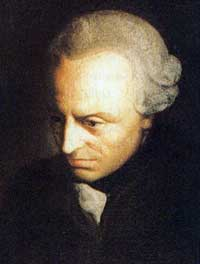
\includegraphics[height=5cm]{../../graphics/kant.jpg}
                \end{center}
            \end{column}
            \begin{column}{0.5\textwidth}
                \begin{center}
                	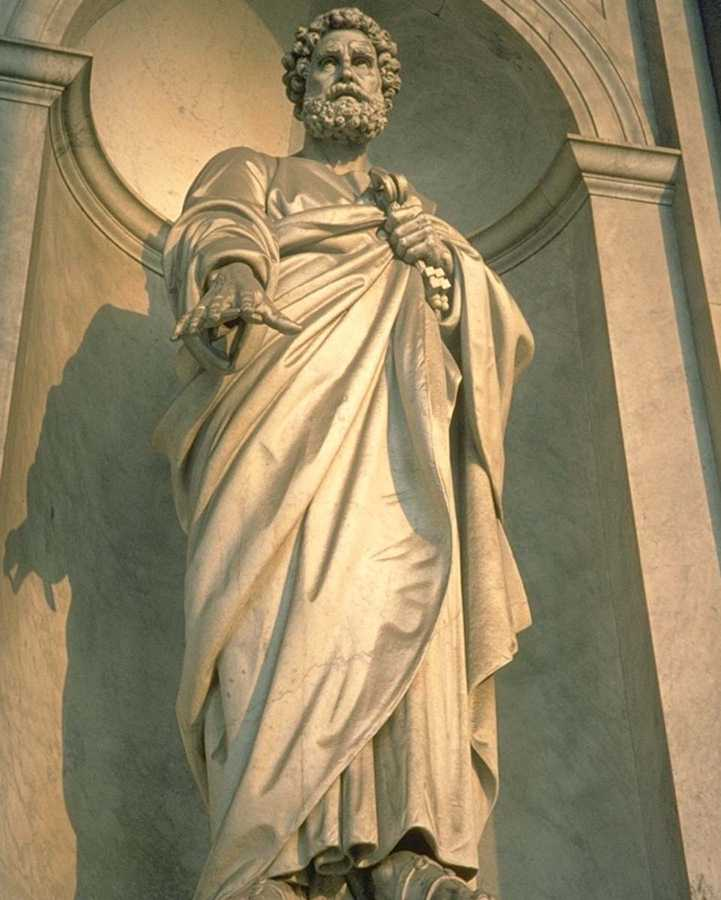
\includegraphics[height=5cm]{../../graphics/socrates.jpg}
                \end{center}
            \end{column}
        \end{columns}
}

Despite conforming to common rational moral cognition, Kant’s claims about the unconditional value of the good will can seem extreme. To allay any doubts, Kant provides a supplementary argument.

The argument appeals to a teleological conception of nature:

\begin{quote}
	Nature endows its creatures with no capacity, even reason, unless that capacity is best suited to achieving its purpose.
\end{quote}

What is the purpose of reason? Not to secure happiness. Nature could have secured that purpose more reliably by endowing us with the appropriate instincts.

Nature endows us with reason, not for the purpose of achieving happiness, but for the purpose of achieving a good will. Reason is a practical capacity—it influences the will. So in a world where nature distributes its endowments in a purposive manner, the purpose of having reason must be to produce a will that is good. The argument is not demonstrative. Nothing in it rules out the possibility of their being other candidate purposes, but Kant things that having eliminated the purpose of happiness, he has eliminated the only relevant alternative.

Kant draws an important distinction between the highest good and the complete good. The good will is the highest good given that it is the indispensable condition of the value of all other goods. The good will’s enjoying the happiness appropriate to it is the complete good. The good will is not the complete good since a person can have a good will without being happy. Nevertheless nature can attain its highest purpose by endowing us with the capacity for achieving a good will even if the likelihood of achieving its second purpose, happiness, were ``less than zero''.

This discussion complements the Pietist theme in Kant’s moral philosophy. Nature endows us with reason for the purpose of achieving a good will. A good will, unlike other kinds of goods, is not a \emph{gift}, it is something to be achieved through the exercise of reason.

The discussion also highlights the potential limits of Kant’s strategy. Kant claims to begin with common rational moral cognition, but the appeal to a teleological conception of nature surely goes beyond this basis. Though perhaps this is just another manifestation of Kant’s Pietism, that is, the way in which unreflective, practical knowledge of rational standards must be supplemented by a reflective, theoretical knowledge in order to avoid corruption and resist temptation.

% \textbf{See Figure~\ref{fig:slide8}.}
% 
% \begin{figure}[ht]
%     \begin{center}
%         \includeslide[height=5cm]{slide8<1>}
%     \end{center}
%     \caption{The Purpose of Reason}
%     \label{fig:slide8}
% \end{figure}

\frame<presentation>[label=slide8]{
    \frametitle{The Purpose of Reason}
        \begin{columns}
            \begin{column}{3cm}
                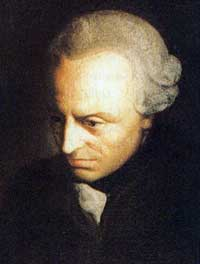
\includegraphics[height=4cm]{../../graphics/kant.jpg}
            \end{column}
            \begin{column}{7cm}
                \begin{itemize}
                    \item \alert{Teleological Conception of Nature}: Nature endows its creatures with no capacity unless that capacity is best suited to achieving its purpose
                    \item Nature endows us with reason not to secure happiness but for the purpose of achieving a good will
                    \item The \alert{highest good} versus the \alert{complete good}
                \end{itemize}
            \end{column}
        \end{columns}
}

% section the_value_of_the_good_will (end)

\end{document}
